\documentclass[draftclsnofoot,onecolumn]{IEEEtran}
\usepackage{url}
\usepackage{listings}  
\usepackage[pdftex]{graphicx}
\usepackage[caption=false,font=footnotesize]{subfig}

%Configure graphicx package
\graphicspath{{./images/}}
\DeclareGraphicsExtensions{.jpeg,.png}

%Configure the lstlisting package https://en.wikibooks.org/wiki/LaTeX/Source_Code_Listings#Using_the_listings_package
\lstdefinestyle{cSharp}{
	language=[Sharp]C, 
	basicstyle=\small\ttfamily, 
	lineskip={-0.1pt},
	tabsize=4,
	aboveskip=15pt,
	belowskip=0pt,
	escapechar=@,
    numbers=left
}
\lstMakeShortInline`

% The IEEEtrans section headers do not make sence for us since we want our requrments to have numbers
\renewcommand\thesection{\arabic{section}}
\renewcommand\thesubsection{\thesection.\arabic{subsection}}
\renewcommand\thesubsubsection{\thesubsection.\arabic{subsubsection}}

\renewcommand\thesectiondis{\arabic{section}}
\renewcommand\thesubsectiondis{\thesectiondis.\arabic{subsection}}
\renewcommand\thesubsubsectiondis{\thesubsectiondis.\arabic{subsubsection}}

% Example of Constructing an image figure: (change label to unique identifier)
%\begin{figure}[!t]
%\centering
%\includegraphics[width=\textwidth]{myfigure}
%\caption{Simulation results for the network.}
%\label{fig_sim}
%\end{figure}

% Example of Constructing a code example figure: (change label to unique identifier)
%\begin{figure}[!t]
%\centering
%\begin{lstlisting}
%public class Logger
%{
%	public virtual void Log(Log log)
%	{
%		Console.WriteLine(log);
%	}
%	public virtual void LogAll(IEnumerable<Log> logs)
%	{
%		foreach(var l in logs)
%		{
%			Log(l);
%		}
%	}
%}
%\end{lstlisting}
%\caption{Simulation results for the network.}
%\label{fig_sim1}
%\end{figure}

% Exapmle of refering to figure
% Blah, blah, and here is Figure \ref{fig_sim}

\begin{document}
\lstset{style=cSharp}
\title{Semantic Diff via C\# Compiler Platform}
%\IEEEspecialpapernotice{Group 19 Winter 2016 Progress Report}

\author{Shawn Fontaine, Cody Ray Hoeft, Michael Rose\\
	School of Electrical Engineering and Computer Science\\
	Oregon State University
\thanks{Group 19 Winter 2016 Progress Report}
\thanks{Proposer/Client: Philip Carter of Microsoft.}}

\maketitle
\pagenumbering{gobble} %removes page number

\begin{abstract}
Lorem ipsum dolor sit amet, consectetur adipiscing elit. Ut aliquam auctor ligula at cursus. Nunc pretium, nulla sit amet sagittis volutpat, leo nisl luctus nibh, eu vehicula lorem leo quis diam. Phasellus in arcu vel felis tincidunt maximus in nec arcu. Phasellus neque lacus, malesuada non pulvinar sed, ornare et ex. Phasellus id suscipit purus, molestie egestas est. Nam placerat vel ex a ultricies. Praesent eros nisl, suscipit sit amet laoreet nec, rhoncus sit amet purus. Pellentesque semper quis ligula nec luctus. Sed ac odio porta, scelerisque risus in, fringilla libero. Pellentesque at vestibulum felis. Aliquam condimentum dapibus maximus. Pellentesque nec velit vel dolor dignissim iaculis sit amet auctor justo. Quisque commodo nunc nec ipsum rutrum, dignissim faucibus ligula vulputate. Sed bibendum dui tellus. Sed laoreet ut enim sit amet condimentum. Proin eget tortor dapibus, ultricies ligula sed, eleifend velit. Maecenas sit amet erat velit. Donec eu finibus mi. Aenean aliquam eleifend tellus. Aliquam pulvinar, dolor in fringilla lacinia, felis lacus iaculis elit, nec mattis risus velit eu lacus. Nunc blandit augue vel lorem eleifend, a fringilla enim condimentum cras amet.
\end{abstract}

\newpage
\setcounter{tocdepth}{2}
\tableofcontents
\newpage
\pagenumbering{arabic}
\section{Introduction}
\subsection{Overview}
Lorem ipsum dolor sit amet, consectetur adipiscing elit. Mauris felis lacus, fringilla et quam sit amet, pellentesque pulvinar leo. Curabitur venenatis, augue sed volutpat sodales, risus ante facilisis mauris, a dictum dui est non quam. Praesent eu tempus justo. Sed vitae urna ultricies, semper urna at, pharetra augue. Etiam pulvinar pharetra leo, sit amet mollis diam lacinia ac. Fusce vitae volutpat neque. Nam mi nulla, luctus eget vehicula sed, scelerisque nec sapien. Lorem ipsum dolor sit amet, consectetur adipiscing elit. Maecenas in arcu eros. Suspendisse convallis nibh nec sapien nullam.

\subsection{Background}
Lorem ipsum dolor sit amet, consectetur adipiscing elit. Mauris felis lacus, fringilla et quam sit amet, pellentesque pulvinar leo. Curabitur venenatis, augue sed volutpat sodales, risus ante facilisis mauris, a dictum dui est non quam. Praesent eu tempus justo. Sed vitae urna ultricies, semper urna at, pharetra augue. Etiam pulvinar pharetra leo, sit amet mollis diam lacinia ac. Fusce vitae volutpat neque. Nam mi nulla, luctus eget vehicula sed, scelerisque nec sapien. Lorem ipsum dolor sit amet, consectetur adipiscing elit. Maecenas in arcu eros. Suspendisse convallis nibh nec sapien nullam.

Lorem ipsum dolor sit amet, consectetur adipiscing elit. Mauris felis lacus, fringilla et quam sit amet, pellentesque pulvinar leo. Curabitur venenatis, augue sed volutpat sodales, risus ante facilisis mauris, a dictum dui est non quam. Praesent eu tempus justo. Sed vitae urna ultricies, semper urna at, pharetra augue. Etiam pulvinar pharetra leo, sit amet mollis diam lacinia ac. Fusce vitae volutpat neque. Nam mi nulla, luctus eget vehicula sed, scelerisque nec sapien. Lorem ipsum dolor sit amet, consectetur adipiscing elit. Maecenas in arcu eros. Suspendisse convallis nibh nec sapien nullam.

Lorem ipsum dolor sit amet, consectetur adipiscing elit. Mauris felis lacus, fringilla et quam sit amet, pellentesque pulvinar leo. Curabitur venenatis, augue sed volutpat sodales, risus ante facilisis mauris, a dictum dui est non quam. Praesent eu tempus justo. Sed vitae urna ultricies, semper urna at, pharetra augue. Etiam pulvinar pharetra leo, sit amet mollis diam lacinia ac. Fusce vitae volutpat neque. Nam mi nulla, luctus eget vehicula sed, scelerisque nec sapien. Lorem ipsum dolor sit amet, consectetur adipiscing elit. Maecenas in arcu eros. Suspendisse convallis nibh nec sapien nullam.

Lorem ipsum dolor sit amet, consectetur adipiscing elit. Mauris felis lacus, fringilla et quam sit amet, pellentesque pulvinar leo. Curabitur venenatis, augue sed volutpat sodales, risus ante facilisis mauris, a dictum dui est non quam. Praesent eu tempus justo. Sed vitae urna ultricies, semper urna at, pharetra augue. Etiam pulvinar pharetra leo, sit amet mollis diam lacinia ac. Fusce vitae volutpat neque. Nam mi nulla, luctus eget vehicula sed, scelerisque nec sapien. Lorem ipsum dolor sit amet, consectetur adipiscing elit. Maecenas in arcu eros. Suspendisse convallis nibh nec sapien nullam.

Lorem ipsum dolor sit amet, consectetur adipiscing elit. Mauris felis lacus, fringilla et quam sit amet, pellentesque pulvinar leo. Curabitur venenatis, augue sed volutpat sodales, risus ante facilisis mauris, a dictum dui est non quam. Praesent eu tempus justo. Sed vitae urna ultricies, semper urna at, pharetra augue. Etiam pulvinar pharetra leo, sit amet mollis diam lacinia ac. Fusce vitae volutpat neque. Nam mi nulla, luctus eget vehicula sed, scelerisque nec sapien. Lorem ipsum dolor sit amet, consectetur adipiscing elit. Maecenas in arcu eros. Suspendisse convallis nibh nec sapien nullam.Lorem ipsum dolor sit amet, consectetur adipiscing elit. Mauris felis lacus, fringilla et quam sit amet, pellentesque pulvinar leo. Curabitur venenatis, augue sed volutpat sodales, risus ante facilisis mauris, a dictum dui est non quam. Praesent eu tempus justo. Sed vitae urna ultricies, semper urna at, pharetra augue. Etiam pulvinar pharetra leo, sit amet mollis diam lacinia ac. Fusce vitae volutpat neque. Nam mi nulla, luctus eget vehicula sed, scelerisque nec sapien. Lorem ipsum dolor sit amet, consectetur adipiscing elit. Maecenas in arcu eros. Suspendisse convallis nibh nec sapien nullam.

Lorem to figure \ref{fig_sim1} or \ref{fig_sim2} ipsum dolor sit amet, consectetur adipiscing elit. Mauris felis lacus, fringilla et quam sit amet, pellentesque pulvinar leo. Curabitur venenatis, augue sed volutpat sodales, risus ante facilisis mauris, a dictum dui est non quam. Praesent eu tempus justo. Sed vitae urna ultricies, semper urna at, pharetra augue. Etiam pulvinar pharetra leo, sit amet mollis diam lacinia ac. Fusce vitae volutpat neque. Nam mi nulla, luctus eget vehicula sed, scelerisque nec sapien. Lorem ipsum dolor sit amet, consectetur adipiscing elit. Maecenas in arcu eros. Suspendisse convallis nibh nec sapien nullam.

\begin{figure}[!t]
\centering
\begin{lstlisting}
public class Logger
{
	public virtual void Log(Log log)
	{
		Console.WriteLine(log);
	}
	public virtual void LogAll(IEnumerable<Log> logs)
	{
		foreach(var l in logs)
		{
			Log(l);
		}
	}
}
\end{lstlisting}
\caption{Simulation results for the network.}
\label{fig_sim1}
\end{figure}


\begin{figure}[!t]
\centering
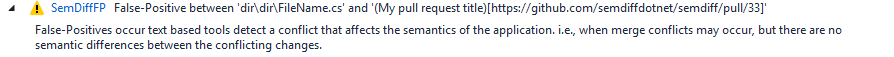
\includegraphics[width=\linewidth]{falsePositiveWarning}
\caption{Simulation results for the network.}
\label{fig_sim2}
\end{figure}


\begin{figure}[!t]
\centering
\begin{itemize}
    \item One
    \item Two
    \item Three
\end{itemize}
\caption{Simulation results for the network.}
\label{fig_sim3}
\end{figure}

\begin{figure}[!t]
\centering
\begin{enumerate}
    \item One
    \item Two
    \item Three
\end{enumerate}
\caption{Simulation results for the network.}
\label{fig_sim4}
\end{figure}


\subsection{Project Purpose and Goals}
Lorem ipsum dolor sit amet, consectetur adipiscing elit. Mauris felis lacus, fringilla et quam sit amet, pellentesque pulvinar leo. Curabitur venenatis, augue sed volutpat sodales, risus ante facilisis mauris, a dictum dui est non quam. Praesent eu tempus justo. Sed vitae urna ultricies, semper urna at, pharetra augue. Etiam pulvinar pharetra leo, sit amet mollis diam lacinia ac. Fusce vitae volutpat neque. Nam mi nulla, luctus eget vehicula sed, scelerisque nec sapien. Lorem ipsum dolor sit amet, consectetur adipiscing elit. Maecenas in arcu eros. Suspendisse convallis nibh nec sapien nullam.





\subsection{Overall Progress}

\subsubsection{Fall Term}
Lorem ipsum dolor sit amet, consectetur adipiscing elit. Mauris felis lacus, fringilla et quam sit amet, pellentesque pulvinar leo. Curabitur venenatis, augue sed volutpat sodales, risus ante facilisis mauris, a dictum dui est non quam. Praesent eu tempus justo. Sed vitae urna ultricies, semper urna at, pharetra augue. Etiam pulvinar pharetra leo, sit amet mollis diam lacinia ac. Fusce vitae volutpat neque. Nam mi nulla, luctus eget vehicula sed, scelerisque nec sapien. Lorem ipsum dolor sit amet, consectetur adipiscing elit. Maecenas in arcu eros. Suspendisse convallis nibh nec sapien nullam.

\subsubsection{Winter Term (Mid)}
Lorem ipsum dolor sit amet, consectetur adipiscing elit. Mauris felis lacus, fringilla et quam sit amet, pellentesque pulvinar leo. Curabitur venenatis, augue sed volutpat sodales, risus ante facilisis mauris, a dictum dui est non quam. Praesent eu tempus justo. Sed vitae urna ultricies, semper urna at, pharetra augue. Etiam pulvinar pharetra leo, sit amet mollis diam lacinia ac. Fusce vitae volutpat neque. Nam mi nulla, luctus eget vehicula sed, scelerisque nec sapien. Lorem ipsum dolor sit amet, consectetur adipiscing elit. Maecenas in arcu eros. Suspendisse convallis nibh nec sapien nullam.

\subsubsection{Winter Term (Final)}










\section{Project Progress}
Lorem ipsum dolor sit amet, consectetur adipiscing elit. Mauris felis lacus, fringilla et quam sit amet, pellentesque pulvinar leo. Curabitur venenatis, augue sed volutpat sodales, risus ante facilisis mauris, a dictum dui est non quam. Praesent eu tempus justo. Sed vitae urna ultricies, semper urna at, pharetra augue. Etiam pulvinar pharetra leo, sit amet mollis diam lacinia ac. Fusce vitae volutpat neque. Nam mi nulla, luctus eget vehicula sed, scelerisque nec sapien. Lorem ipsum dolor sit amet, consectetur adipiscing elit. Maecenas in arcu eros. Suspendisse convallis nibh nec sapien nullam.






\subsection{Query GitHub for Pull Request}

\textbf{Requirement:}

\begin{quote}

SemDiff will query the GitHub repo cloned in VS for pull request and the files changed.

\end{quote}

\subsubsection{Progress}

\subsubsection{Methodology}

\subsubsection{Future Work}

\subsubsection{Problems}






\subsection{False-Positive Detection}

\textbf{Requirement:}

\begin{quote}

SemDiff will detect changes between two version of a file that will cause a text-based merge conflict but do not change the semantics of the code. This is defined as a false-positive. This will require at least partial completion of requirement 1, because we will need to know the format/state that we will receive files.

\end{quote}

\subsubsection{Progress}

\subsubsection{Methodology}

\subsubsection{Future Work}

\subsubsection{Problems}






\subsection{False-Negative Detection}

\textbf{Requirement:}

\begin{quote}

SemDiff will detect if the underlying methods used by another method have been semantically changed given a set of files that have been changed by another developer. This is defined as a false-negative). This will require at least partial completion of requirement 0, because we will need to know the format/state that we will receive files.

\end{quote}

\subsubsection{Progress}

\subsubsection{Methodology}

\subsubsection{Future Work}

\subsubsection{Problems}






\subsection{Displaying False-Positive Warnings in Error List}

\textbf{Requirement:}

\begin{quote}

At compile time, SemDiff will display a warning in the “Error List” when a false-positive occurs between local files and remote files retrieved from a pull request. This will require requirements 1 and 2 because the files and the functionality to compare will be needed.

We will show that a false-positive was detected.

We will show the name of the file in conflict.

We will provide a link to the pull request.

\end{quote}

\subsubsection{Progress}

\subsubsection{Methodology}

\subsubsection{Future Work}

\subsubsection{Problems}






\subsection{Displaying False-Negatives Warnings in Error List}

\textbf{Requirement:}

\begin{quote}

SemDiff will display a warning in the “Error List” (at compile time) when a false-negative occurs between the semantics of the classes represented by the local files and the classes represented by the remote files retrieved from a pull request. This will require requirements 0 and 0 because the files and functionality to semantically diff will be needed.

We will show that a false-negative was detected.

We will show which classes are in conflict.

We will show which classes are in conflict.

We will provide a link to the pull request.

\end{quote}

\subsubsection{Progress}

\subsubsection{Methodology}

\subsubsection{Future Work}

\subsubsection{Problems}






\subsection{NuGet Package}

\textbf{Requirement:}

\begin{quote}

SemDiff will provide a NuGet package that can be installed to a VS project as an Analyzer.

\end{quote}

\subsubsection{Progress}

\subsubsection{Methodology}

\subsubsection{Future Work}

\subsubsection{Problems}






\subsection{Performance}

\textbf{Requirement:}

\begin{quote}

SemDiff will minimally impact VS performance.

\end{quote}

\subsubsection{Progress}

\subsubsection{Methodology}

\subsubsection{Future Work}

\subsubsection{Problems}






\subsection{Informative Alerts}

\textbf{Requirement:}

\begin{quote}

Alerts will be informative

\end{quote}

\subsubsection{Progress}

\subsubsection{Methodology}

\subsubsection{Future Work}

\subsubsection{Problems}






\subsection{GitHub Project Hosting}

\textbf{Requirement:}

\begin{quote}

All source code, documentation, and issue tracking should be hosted publicly on GitHub. The GitHub wiki shall contain documentation for the project including a Getting Started guide, an API Guide with code examples, and motivational purpose of the project.

\end{quote}

\subsubsection{Progress}

\subsubsection{Methodology}

\subsubsection{Future Work}

\subsubsection{Problems}






\subsection{MIT Licensing}

\textbf{Requirement:}

\begin{quote}

All outputs of the project should be open source and licensed with the MIT license.

\end{quote}






\subsection{Documentation in Code}

\textbf{Requirement:}

\begin{quote}

Source code will contain header comments on public classes, public interfaces, and public methods. Methods will only contain comments that help explain the function of obscure code.

\end{quote}

\subsubsection{Progress}

\subsubsection{Methodology}

\subsubsection{Future Work}

\subsubsection{Problems}






\subsection{Development Technology}

\textbf{Requirement:}

\begin{quote}

SemDiff will be built using C\# and the Roslyn API.

\end{quote}

\subsubsection{Progress}

\subsubsection{Methodology}

\subsubsection{Future Work}

\subsubsection{Problems}










\section{Conclusion}

Lorem ipsum dolor sit amet, consectetur adipiscing elit. Mauris felis lacus, fringilla et quam sit amet, pellentesque pulvinar leo. Curabitur venenatis, augue sed volutpat sodales, risus ante facilisis mauris, a dictum dui est non quam. Praesent eu tempus justo. Sed vitae urna ultricies, semper urna at, pharetra augue. Etiam pulvinar pharetra leo, sit amet mollis diam lacinia ac. Fusce vitae volutpat neque. Nam mi nulla, luctus eget vehicula sed, scelerisque nec sapien. Lorem ipsum dolor sit amet, consectetur adipiscing elit. Maecenas in arcu eros. Suspendisse convallis nibh nec sapien nullam.










\section{Glossary}

\begin{description}[\IEEEsetlabelwidth{NuGet Package:}\IEEEusemathlabelsep] %The label width should be the longest term

\item[.NET:] Framework that provides the runtime and core libraries for C\# and other languages

\item[AST:] Abstract Syntax Tree is a parsed data structure that represents all of the tokens in source code.

\item[C\#:] Refers to C\# 6.0. Programming language that we are targeting. See https://goo.gl/y6A13i.

\item[Diff:] Tool that compares two versions of code to look for changes.

\item[False-Positive:] Error that occurs when one developer writes code that calls a function and creates a pull request while another developer creates a semantic change in the function that the previous developer depends on. This can change the actual functionality to differ from what is expected by the first developer even though the changes may merge (using text based tools) without warning. This can create subtle runtime bugs that can be difficult to detect. A false-positive is not caught by text-based diff software.

\item[False-Negative:] Errors that occur when one developer makes a non-semantic change (i.e., moves a function) and another makes a semantic change that conflicts (i.e., edits the contents of the function). When the pull request is merged (using text based tools), it will result in conflict even though semantic changes were only created by the latter developer.

\item[GitHub:] Website that provide version control, issue tracking, and documentation tools for software projects

\item[NuGet Package:] Open-source package manager for the Microsoft development platform. Provides the ability to produce and consume package in Visual Studio.

\item[Roslyn:] “Roslyn provides open-source C\# and Visual Basic compilers with rich code analysis APIs. It enables building code analysis tools with the same APIs that are used by Visual Studio.” – Roslyn Readme 

\item[Semantics:] Semantics of a program represent the executing behavior and the meaning/purpose of what is being executed. 

\item[VS:] Popular IDE for working with C\#, when used here it refers to Visual Studio 2015

\end{description}

See \url{https://help.github.com/articles/github-glossary/} for git and GitHub related terminology

\end{document}
